\subsection{Berechnung}
Um einen Ball durch die Schwungräder mit einem gewissen Anpressdruck zu führen, wird ein
Drehmoment benötigt. Dazu wird der Tennisball als eine Feder mit der Federkonstante k betrachtet. Zur Ermittlung von k wurde der Ball mit einer Masse m
beschwert, und die Verschiebung x gemessen.

\begin{figure}[h!]
	\centering
	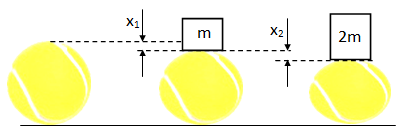
\includegraphics[width=0.6\textwidth]{Enddokumentation/Anhang/Bilder/KompressionBaelle.png}
	\caption{Bestimmung von k}
	\label{fig:BallKomp}
\end{figure}

\begin{table}[h!]
	\begin{tabular}{p{1.5cm}p{1.7cm}}
		Gewicht & Auslenkung\\
		\hline
		1kg & 1 mm\\
		2kg & 2 mm\\
		3kg & 3 mm\\
	\end{tabular}
	\centering
	\caption{Prinzip der k-Bestimmung}
	\label{tab:BallKompErgebnis}
\end{table}

Da $x_1$ und $x_2$ in etwa gleich gross sind, kann von einer linearen Federkonstante
ausgegangen werden. Damit kann die Kraft, die durch das Stauchen des Balles entsteht mit der
Formel

\begin{equation}  
    F_s=2\cdot k \cdot \Delta x 
\end{equation}

bestimmt werden. Die Federkonstante k beträgt $9.8\frac{N}{mm}$ Das entstehende Drehmoment,
wird mit trigonometrischer Beziehung hergeleitet.
\begin{align}  
    \label{equ:Formel_M} %Muss hier sein, damit die Referenz zur ersten Formel zeigt.
    M &= R_S \cdot F_t\\
    F_t &= F_s \cdot \sin(\alpha)\\ 
    F_s &= 2\cdot k \cdot \Delta x 
\end{align}

\begin{figure}[h!]
	\centering
	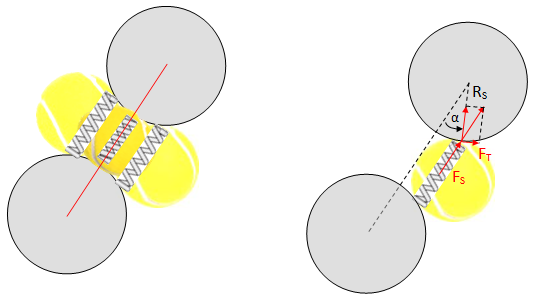
\includegraphics[width=0.4\textwidth]{Enddokumentation/Anhang/Bilder/PrinzipKompression.png}
	\caption{Prinzip der Kompression}
	\label{fig:PrinzipBallKomp}
\end{figure}

\begin{wrapfigure}{r}{0.3\textwidth}
    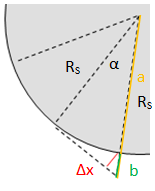
\includegraphics[scale=0.75]{Enddokumentation/Anhang/Bilder/GrafikKreisErkaerung.png}
    \centering
    \caption{keine Ahnung}
    \label{abb:KreisErkaerung}
\end{wrapfigure}
Da $\Delta x$ vom Winkel $\alpha$ abhängt, siehe Abbildung \ref{abb:KreisErkaerung} muss die
folgende Abhängigkeit gelten:
\begin{equation}  
	\alpha = R_s \cdot \frac{1}{\cos(\alpha)} \\ \lvert \\ b = a - R_s = R_s \left( \frac{1}{\cos(\alpha)}-1\right)   
\end{equation}

\begin{equation}
	\Delta x = b \cdot \cos(\alpha) = R_a \cdot \left[1 - \cos(\alpha)\right]
\end{equation}

Somit gilt:
\begin{equation} 	\Delta x =  R_s \cdot \left[1 - \cos(\alpha)\right]
	\label{equ:Formel_DeltaX}
\end{equation}

Fügt man nun die Formeln \ref{equ:Formel_M} bis \ref{equ:Formel_DeltaX} zusammen erhält man
das Drehmoment in Abhängigkeit zum Winkel:
\begin{equation}  
    M = 2 \cdot R_s{^{2}} \cdot k \cdot \left[1 - \cos(\alpha)\right] \cdot \sin(\alpha)\\\lvert\\ \left[ |a| \leq \arccos \left(1-\frac{1}{R_s}\right)\right]
\end{equation}
Berechnet mit den Werten $R_s = 40 mm$, $k = 9.8 \frac{N}{mm}$, $L = 146 mm$ und
$DBall = 68 mm$ ergibt sich der folgende Verlauf über den Winkel. Dabei ist ersichtlich,
dass sich das Maximum jeweils beim Grenzwinkel liegt. Dort wird das Drehmoment bei 0 liegen,
da keine Kraft angreift. Der Betrag des maximalen Drehmoments liegt bei $0.174 Nm$ und einem
Winkel von $12.84^\circ$.

\begin{figure}[h!]
	\centering
	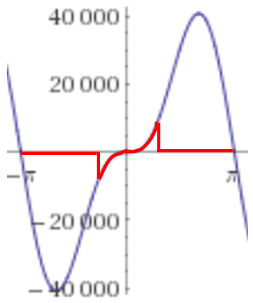
\includegraphics[width=0.3\textwidth]{Enddokumentation/Anhang/Bilder/WeissNicht.png}
	\caption{keine Ahnung}
	\label{fig:keineAhnung}
\end{figure}
Die kurzzeitige Laständerung durch den Abwurf eines Balles kann aufgrund der Trägheit des
Motors nicht ausgeglichen werden. Deshalb soll eine Energiebilanz Aufschlüsse über den
Drehzahlverlust geben. Der Ball hat zwischen den Punkten 0 und 1 zwei verschiedene Energien.
Eine potentielle sowie eine kinetische Energie. Zusätzlich besitzen die Schwungräder
aufgrund ihrer Trägheit eine Rotationsenergie.
\begin{align}
 	&\sum E_{pot} &+&& \sum E_{kin} &&+&& \sum E_{rot} &= 0 \\
 	& m_{ball} \cdot \left(h_1 - h_0\right) &+&&\frac{1}{2} \cdot \left( v_1{^{2}} - v_0{^{2}} \right) &&+&&\frac{1}{2} \cdot J \left( \omega_1{^{2}} - \omega_0{^{2}} \right) &= 0
\end{align}

Die Berechnung der Anfangsgeschwindigkeit des Balles ist von der Zuführgeschwindigkeit wie
folgt abhängig:
\begin{equation}
 	v_0 = v_{band} \cdot \cos(\beta)
\end{equation}

Die Endgeschwindigkeit kommt aufgrund des schiefen Wurfes zustande
\begin{figure}[h!]
	\centering
	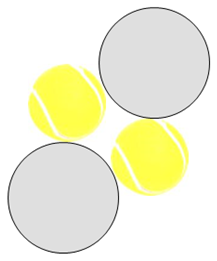
\includegraphics[width=0.3\textwidth]{Enddokumentation/Anhang/Bilder/Ballnachfuehrung.png}
	\caption{keine Ahnung}
	\label{fig:Ballnachführung}
\end{figure}

Das Trägheitsmoment beträgt
\begin{equation}
 	J = \sum_{i}^{N} m_ir_i{^{2}}
\end{equation}

Somit ist eine grosse Masse in weitem Abstand zur Achse anzustreben. Es wird das Trägheitsmoment eines Vollzylinders für die Berechnung verwendet. Dieser lautet:
\begin{equation}
 	J = \frac{1}{2} m \cdot r^2
\end{equation}

Die Masse ist dabei 	
\begin{equation}
	m = \rho \cdot V \\\lvert\\ m = \rho \cdot d_{rad} \cdot \pi \cdot b_{rad}
\end{equation}
Das resultierende Trägheitsmoment beträgt $0.00018 kg m^2$\\
\\
\begin{wrapfigure}{r}{0.3\textwidth}
	 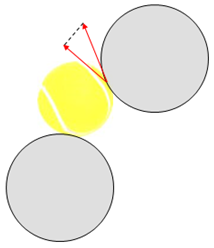
\includegraphics[scale=0.75]{Enddokumentation/Anhang/Bilder/AbwurfBild.png}
	 \centering
	 \caption{keine Ahnung}
	 \label{abb:AbwurfBild}
\end{wrapfigure}
Zwischen der Abwurfgeschwindigkeit und der Winkelgeschwindigkeit gibt es eine Relation.
Dabei wird angenommen, dass der Ball ohne Schlupf die Schwungräder durchläuft. Im
Eintrittspunkt wird der Ball mit einem Sprung beschleunigt. Beim Winkel alpha=0 ist die
Geschwindigkeit am höchsten. Danach wird der Ball wieder abgebremst.
\begin{align}
	v_1 &= v_u \cdot \cos(\alpha)\\
	v_u &= 4\pi \cdot R_s \cdot n_1
\end{align}

Der Höhenunterschied $\delta H$ wird ausgedrückt durch:
\begin{equation}
	\Delta H = \frac{L \cdot \tan(\alpha)}{\sqrt{2}}
\end{equation}

Die Winkelgeschwindigkeiten werden durch die Drehzahl definiert:
\begin{equation}
	\omega = 2\pi \cdot n
\end{equation}

Nun kann die Energiegleichung aufgestellt werden:
\begin{multline}
	m_{Ball} \cdot g \cdot \frac{L \cdot \tan(\alpha)}{\sqrt{2}} + \frac{1}{2} \cdot m_{Ball} \cdot \left(\left[4\pi \cdot R_s \cdot n_1 \cdot \cos(\alpha)\right]^2 - \left[ v_{Band} \cdot \frac{1}{\sqrt{2}}\right]^2\right) +\\
	\frac{1}{2} \cdot J \cdot \left(\left[2\pi \cdot n_1\right]^2 - \left[2\pi \cdot n_0\right]^2\right) = 0
	\label{equ:AbbremsungBall}
\end{multline}
Berechnet mit den gegebenen Werten von: $mBall = 0.055 kg$, $g = 9.81\frac{N}{kg}$, $L = 0.146 m$, $R_s = 0.040 m$, $v_{Band} = 0 \frac{m}{s}$, $J = 0.00018 kgm^2$, $n_0 = 41\frac{U}{s}$, $a = 12.84^\cdot$ ergebt sich eine Drehzahl von $24.2 \frac{U}{s}$. Dies entspricht 58\% der Nenndrehzahl.\\
\\
Verdoppelt man nun das Trägheitsmoment J, so steigt die Nenndrehzahl auf $29.6 \frac{U}{s}$
an. Dies entspricht 71\% der Nenndrehzahl.\\
\\
Als nächstes wird die Zeit für das Beschleunigen der Räder von der abgebremsten Drehzahl
wieder auf die Nenndrehzahl berechnet.
\begin{align}
	M &= \alpha \cdot J\\
	n_0 &= n_1 + \alpha \cdot t
\end{align}
Somit gilt:
\begin{equation}
	t = \frac{n_0 - n_1}{\alpha} = \frac{\Delta n \cdot J}{M}
\end{equation}
Wir setzen nun vereinfacht, für das Trägheitsmoment, dieses des Schwungrades ein. Das Moment
des Motors soll $0.5 Nm$ betragen. Somit resultiert ein t von $6 ms$. 

Um die Abwurfgeschwindigkeit des Balles aus dem Wurfgerät zu bestimmen, wurde der schiefe
Wurf ohne Luftwiderstand berechnet, da für diese Anwendung die Abweichung durch den
Luftwiderstand minimal ist.
\begin{figure}[h!]
	\centering
	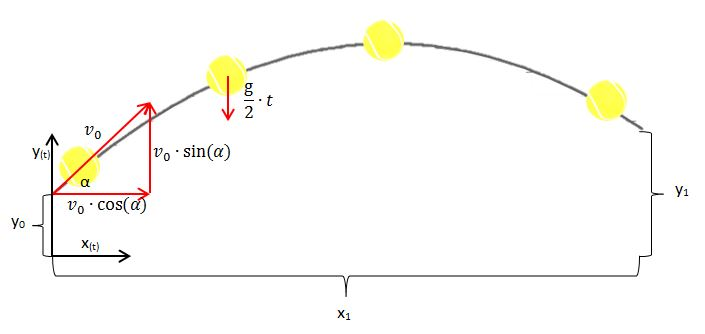
\includegraphics[width=0.9\textwidth]{Enddokumentation/Anhang/Bilder/Schiefer_Wurf2.jpg}
	\caption{Wurfparabel}
	\label{fig:Wurfparabel}
\end{figure}
\begin{align}
	x_{(t)} &= v_0 \cdot \cos(\alpha_0)\\
	y_{(t)} &= y_0 + v_0 \cdot t \cdot \sin(\alpha_0) - \frac{1}{2} \cdot g \cdot t^2
\end{align}

Mit den definierten Werten $x_1 = 1.8 m$, $y_0 = 0.125 m$, $y_1 = 0.4 m$ und 
$g = 9.81 \frac{m}{s}$ ergibt sich eine Zeitdauer von $t = 0.56 s$ und eine
Abwurfgeschwindigkeit von $4.56 \frac{m}{s}$ Die nachfolgende Abbildung
\ref{fig:Wurfparabel1} zeigt die resultierende Wurfparabel.
\begin{figure}[h!]
	\centering
	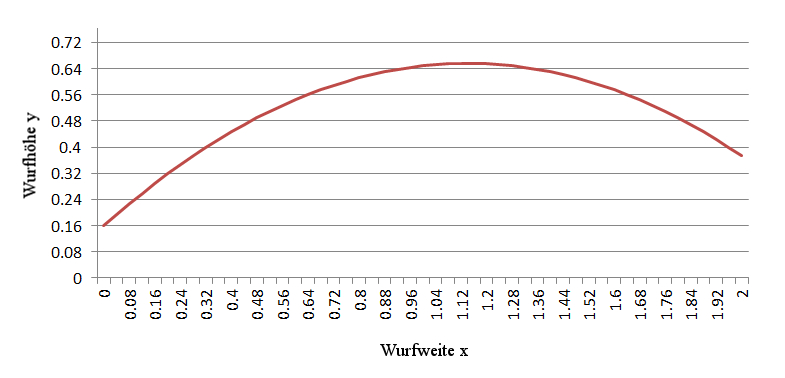
\includegraphics[width=1\textwidth]{Enddokumentation/Anhang/Bilder/Schiefer_Wurf.jpg}
	\caption{Wurfparabel}
	\label{fig:Wurfparabel1}
\end{figure}

\textbf{Berechnung des Drehmoment des Förderbands}\\
%\begin{figure}[h!]
%	\centering
%	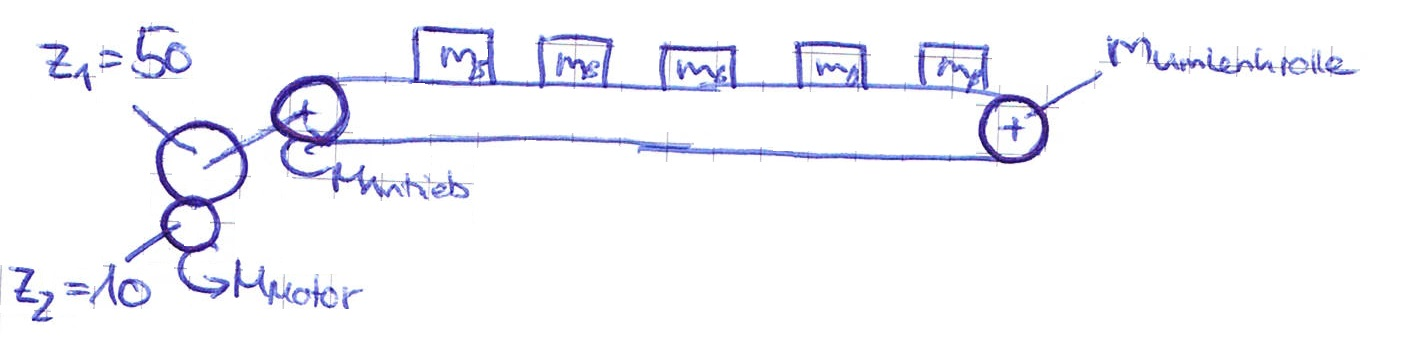
\includegraphics[width=1\textwidth]{Enddokumentation/Anhang/Bilder/FoerderbandSkizze.jpg}
%	\caption{Erläuterungen zur Förderbandberechnung}
%\end{figure}\\

\begin{figure}[h!]
    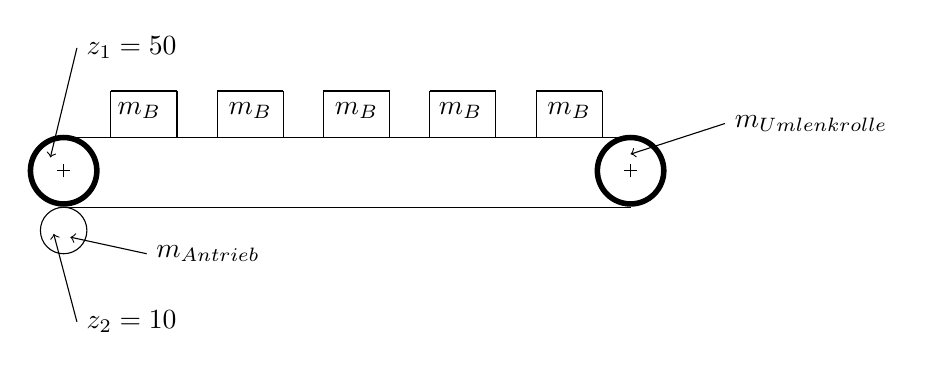
\begin{tikzpicture}[scale = 1.2]
    \draw [-,line width=2pt](0,0) circle (10pt);\draw [-,line width=2pt](6,0) circle (10pt); %beide Kreise der hauptrollen
    \draw  (0,10pt) -- (6, 10pt); \draw (0,-11pt) -- (6,-11pt); %die beiden Förderbänder-Striche
    \draw (0,-2pt) -- (0, 2pt); \draw (0cm-2pt,0) -- (0cm+2pt, 0); %Das x der ersten Rolle
    \draw (6,-2pt) -- (6, 2pt); \draw (6cm-2pt,0) -- (6cm+2pt, 0); %Das x der zweiten Rolle
    \draw [<-] (6cm-0pt , 5pt) -- (7,0.5)node[right]{$m_{Umlenkrolle}$}; %zeige-Linie auf das Hintere Rad mit Text
    \draw (5,10pt) -- (5, 24pt);\draw (5.7,10pt) -- (5.7, 24pt);\draw (5,24pt) -- (5.7, 24pt);\node  at (5.35,18pt) {$m_B$};
    \draw (3.875,10pt) -- (3.875, 24pt);\draw (4.575,10pt) -- (4.575, 24pt);\draw (3.875,24pt) -- (4.575, 24pt);\node  at (4.2,18pt) {$m_B$};
    \draw (2.75,10pt) -- (2.75, 24pt);\draw (3.45,10pt) -- (3.45, 24pt);\draw (2.75,24pt) -- (3.45, 24pt);\node  at (3.1,18pt) {$m_B$};
    \draw (1.625,10pt) -- (1.625, 24pt);\draw (2.325,10pt) -- (2.325, 24pt);\draw (1.625,24pt) -- (2.325, 24pt);\node  at (1.975,18pt) {$m_B$};
    \draw (0.5,10pt) -- (0.5, 24pt);\draw (1.2,10pt) -- (1.2, 24pt);\draw (0.5,24pt) -- (1.2, 24pt);\node  at (.8,18pt) {$m_B$};
    \draw (0,-18pt) circle (7pt);  \draw [<-] (2pt , -20pt) -- (25pt,-25pt)node[right]{$m_{Antrieb}$}; %zeige-Linie auf das Antriebsrad mit Beschriftung
    \draw [<-] (-4pt , 4pt) -- (4pt,1.3)node[right]{$z_1 = 50$}; %zeige-Linie auf das linke Umlenkrad mit Beschriftung
    \draw [<-] (-3pt , -19pt) -- (4pt,-1.6)node[right]{$z_2 = 10$}; %zeige-Linie auf das Antriebsrad mit Beschriftung
    \end{tikzpicture}
   	\centering
    \caption{Erläuterungen zur Förderbandberechnung}
\end{figure}
Formalismus:
\begin{align}
    \label{equ:DrehmomentFörderband}
    M_{Motor} &= M_{Antrieb} \cdot i\\
    i &=\frac{Z_1}{Z_2}\\
    M_{Antrieb} &= F_u \cdot r_A\\
    F_u &= \mu_T \cdot g \cdot \left(5 \cdot m_B + m_{Umlenkrolle} + m_{Band} \right)\\
    M_{Motor} &= \mu \cdot g \cdot r_A \cdot \left(5 \cdot m_B + m_{Umlenkrolle} + m_{Band}\right) \cdot \frac{Z_1}{Z_2}
\end{align}
Verwendete Werte:\\
$\mu_T = 0.33$\\
$g = 9.81\frac{m}{s^2}$\\
$r_A = 0.008 m$\\
$m_B = 0.055 kg$\\
$m_{Umlenkrolle} = 0.020 kg$\\
$m_{Band} = 0.035 kg$\\
$Z_1 = 50$\\
$Z_2 = 10$\\
Daraus ergibt sich ein Drehmoment von $0.0017 Nm$ = \uuline{$1.7 Nmm$}\\
\\
\textbf{Berechnung Drehmoment des Ausrichtungsmechanismus}\\
\begin{wrapfigure}{r}{0.43\textwidth}
	\centering
	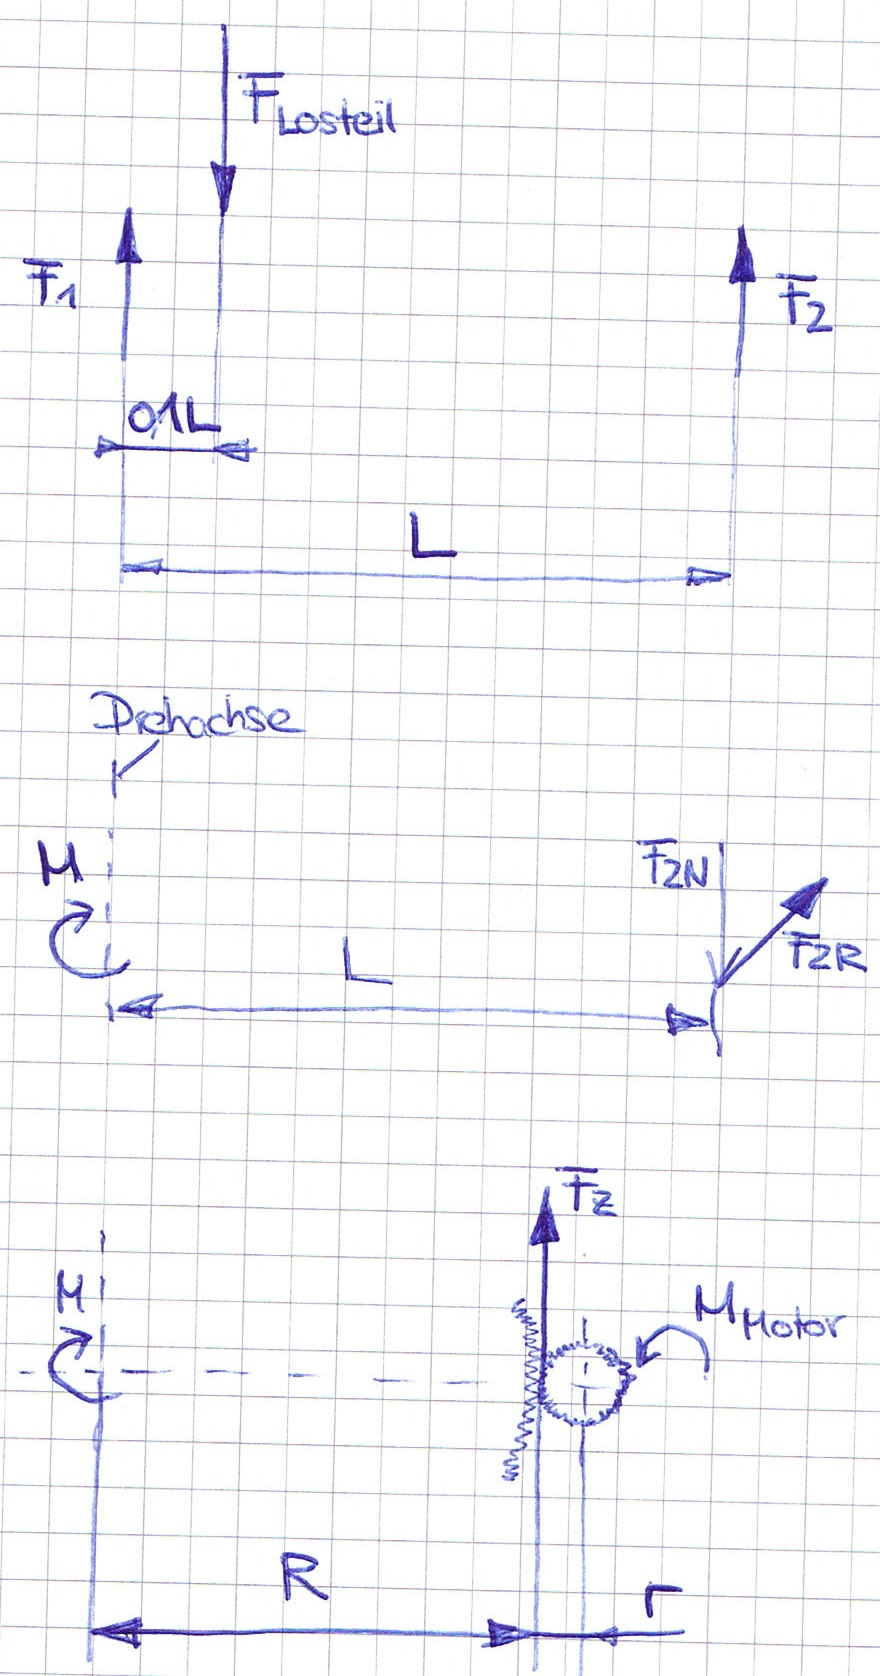
\includegraphics[width=0.45\textwidth]{Enddokumentation/Anhang/Bilder/NotizBerechnungDrehmomentStepper.jpg}
	\caption{Erläuterungen zur Schrittmotorberechnung}	
\end{wrapfigure}
Formalismus:
\begin{align}
    F_{Losteil} &= m_{Losteil} \cdot g\\
    F_2 &= F_{Losteil} \cdot 0.1
\end{align}

\begin{align}
    M_{Drehung} &= L \cdot F_{2R}\\
    F_{2R} &= \mu_H \cdot F_2
\end{align}

\begin{align}
    M_{Motor} &= F_z \cdot r\\
    F_z &= \frac{M_{Drehung}}{R}\\
    M_{Motor} &=\frac{L \cdot \mu_H \cdot m_{Losteil} \cdot g \cdot 0.1}{R} \cdot r
\end{align}
Verwendete Werte:\\
$L = 0.437m$\\
$\mu_H = 0.2$\\
$m_{Losteil} = 1.6 kg$\\
$g = 9.81 \frac{m}{s^2}$\\
$R = 0.28 m$\\
$r = 0.01 m$\\
Daraus ergibt sich ein Drehmoment von \\
$0.0049 Nm$ = \uuline{$4.9 Nmm$}\\
